\documentclass[
    fontsize=12pt,
    paper=a4,
    abstract=false,
    numbers=noenddot,
    listof=totoc,
    bibliography=totoc,
    %twoside,
    %open=right,
    %cleardoublepage=plain,
    parskip=half+
]{scrreprt}

\setcounter{tocdepth}{3}  % Inhaltsverzeichnis bis Subsubsection
\setcounter{secnumdepth}{3} % Nummerierung bis Subsubsection

% General stuff
\usepackage[utf8]{inputenc} % CHANGE HERE IF NECESSARY
\usepackage[T1]{fontenc}
\usepackage[ngerman]{babel} % last language given is used (here: new german)
\usepackage{lmodern}
%\usepackage{microtype}
\usepackage{ifpdf}
\usepackage{ifthen}

% Set date here 
%\day=6 \month=6 \year=2012

% Set name and title
\author{Simon Krempin}
\title{Gegenüberstellung der beiden Programmiersprachen Java und Python, sowie einer praktischen Anwendung von Python}
\date{15. März 2021}

%%%%%% %%%%%%

% Load packages ...
\usepackage{setspace}
\onehalfspacing

\usepackage{geometry}
\geometry{
    left = 4cm,
    right = 2cm,
    top = 2cm,
    bottom = 2cm,
    footskip = 7.5mm
}

\usepackage{mathptmx}
\usepackage{float}

% Corporate Design
\usepackage{eso-pic}
\usepackage{color}
% Comment out if the RUB fonts are installed
% Link: https://noc.rub.de/~jobsanzl/latex/rubtexfonts-0.4.tar.gz
%\usepackage{rubfonts2009} 
\newcommand{\setrubfontnormal}[1]{\fontfamily{rubscala}\fontsize{#1}{1}\selectfont}
\newcommand{\setrubfontextra}[1]{\fontfamily{rubflama}\fontsize{#1}{1}\selectfont}
\definecolor{rubgreen}{cmyk}{0.5,0,1,0}
\definecolor{rubblue}{cmyk}{1,0.5,0,0.6}

% Figures
\usepackage{graphicx}
\usepackage{subfig}
\usepackage{placeins}

% Tables
\usepackage{booktabs}
\usepackage{marvosym}
\usepackage{multirow}

% Math stuff and units
\usepackage{latexsym,amsmath, amssymb, amsfonts, upgreek}
\usepackage{siunitx}
\newcommand{\mathup}{\mathrm}

% Glossary
\usepackage[nonumberlist, acronym, toc]{glossaries}

% Enable quotes by \enquote{}
\usepackage[babel,english=american, german=quotes]{csquotes}

% Necessary for frontpage, allows to create automata and fancy graphics
\usepackage{tikz}

% Protocols and bytefields
% \usepackage{protocol}
\usepackage{bytefield}

% Source code listings
\newcommand{\code}[1]{\texttt{#1}}
\definecolor{colIdentifier}{rgb}{0,0,0}
\definecolor{colComments}{rgb}{0.5,0.5,0.5}
\definecolor{colKeys}{rgb}{0,0,1}
\definecolor{colString}{rgb}{0,0.6,0}

\usepackage{caption}
\usepackage{listings}
\lstset{%
	float=hbp,%
	basicstyle=\ttfamily\scriptsize, %
	identifierstyle=\color{colIdentifier}, %
	keywordstyle=\color{colKeys}, %
	stringstyle=\color{colString}, %
	commentstyle=\color{colComments}, %
	columns=flexible, %
	tabsize=2, %
	aboveskip={1.5\baselineskip}, %
	frame=single, %
	extendedchars=true, %
	showspaces=false, %
	showstringspaces=false, %
	numberstyle=\tiny, %
	breaklines=true, %
	backgroundcolor=, %
	breakautoindent=true, %
	captionpos=b%
}

% Algorithms
\usepackage[ruled, vlined, linesnumbered,algochapter,algo2e]{algorithm2e}
\renewcommand{\listalgorithmcfname}{Algorithmenverzeichnis}

% Format page foot and header
\usepackage{scrlayer-scrpage}
\clearscrheadings
\clearscrheadfoot
\automark[section]{chapter}
\cfoot{\pagemark}
\renewcommand*{\chapterpagestyle}{scrheadings}
\pagestyle{scrheadings}

%% use some standards for mathematical expressions:
\newcommand{\red}{{\rm red}}
\newtheorem{theorem}{Theorem}[section]
\newtheorem{lemma}[theorem]{Lemma}
\newtheorem{proposition}[theorem]{Proposition}
\newtheorem{corollary}[theorem]{Corollary}
% \newtheorem{definition}[theorem]{Definition}
\newtheorem{algorithm}[theorem]{Algorithm}
\newenvironment{example}{\begin{quote}{\bf Example:}}{\end{quote}}

% BIBTEX, http://mirrors.ctan.org/biblio/bibtex/contrib/babelbib/babelbib.pdf
\usepackage{babelbib}
\usepackage{url}
\def\UrlBreaks{\do\/\do-}

% \setbibpreamble{{\large Seitenzahlen, auf denen ein Eintrag referenziert wird, werden am Ende eines jeden Eintrags angegeben.}\newline} % Wegen der pagebackref-Option des hyperref-Packets, wird vielen nicht direkt klar was das soll http://projekte.dante.de/DanteFAQ/Verzeichnisse#16

% gray definition boxes, that whay you'll find them in the text
\usepackage{shadethm}
\newshadetheorem{sthm}[figure]{Definition}
\newenvironment{definition}[1][]{
   \definecolor{shadethmcolor}{rgb}{.9,.9,.9}
   \begin{sthm}[#1]
 }{\end{sthm}}

% experimental
%\usepackage{scrhack}

% Hyperlinks and menu for your document
\usepackage[breaklinks,hyperindex,colorlinks,anchorcolor=black,citecolor=black,filecolor=black,linkcolor=black,menucolor=black,urlcolor=black,pdftex]{hyperref} % pagebackref: Add page number to the references where they can be found
% DO NOT LOAD ANY OF YOUR PACKAGES BEYOND THIS PACKAGE

\makeatletter
\AtBeginDocument{
 \hypersetup{
   pdftitle = {\@title},
   pdfauthor = {\@author},
   pdfsubject={\@title},
   pdfkeywords={SAML, add more}, % CHANGE HERE
%    unicode={true},
 }
}
\makeatother

% Use the same counter for tables and figures
\makeatletter
\AtBeginDocument{
\let\c@table\c@figure
\let\c@lstlisting\c@table
\let\c@algocf\c@lstlisting
}
\makeatother

\ifpdf
	\hypersetup{linktocpage=false} 	% false=links are section names, true=links are page numbers, IMPORTANT: in dvi2ps mode, 'true' is required!
\else
	\hypersetup{linktocpage=true} 		% false=links are section names, true=links are page numbers, IMPORTANT: in dvi2ps mode, 'true' is required!
	\usepackage[hyphenbreaks]{breakurl}
\fi


\begin{document}

    \begin{titlepage}
	\centering
	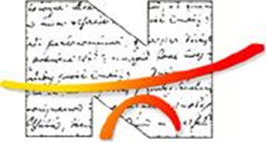
\includegraphics[width=0.4\textwidth]{images/logo.png}\par\vspace{1cm}
	{\scshape\LARGE Nepomucenum Coesfeld \par}
	\vspace{1cm}
	{\scshape\Large erweiterte Lernleistung Informatik\par}
	\vspace{1.5cm}
	{\huge\bfseries Konzeptionierung und Entwicklung einer Anwendung für Schülern basierend auf Spaced Repetition\par}
	\vspace{2cm}
	{\Large\itshape Simon Krempin\par}
	\vfill
	Begleitender Lehrer\par
	\textsc{Jens Brumma}

	\vfill

% Bottom of the page
	{\large 6. April 2022\par}
\end{titlepage}
\clearpage
%\pagestyle{scrheadings}
\tableofcontents
\pagenumbering{gobble}
\clearpage

    \pagenumbering{arabic}
\setcounter{page}{3}
\chapter{Einleitung}
In der Schule wird täglich gelernt, dennoch wird oftmals nicht gelernt, wie man lernt. Ein Schüler muss selber herausfinden, wie er relevante Informationen möglichst zeiteffizient und detailliert beibehält. Aber gerade die richtigen Lernmethoden machen oft den Unterschied zwischen guten und schlechten Schülern aus \cite{OECD:Lernen}\cite{Hattie:Einflussfaktoren}. Es ist daher essenziell diese Unterschiede auszugleichen und damit einen Beitrag für eine größere Chancengleichheit zu leisten. Im besten Fall sorgt eine Verbesserung der Lernmethoden langfristig zu einem, wenn auch nur minimalen, höheren Wissensniveau.

Es ist nicht erst seit der von Ebbinghaus formulierten Forgetting Curve bekannt, dass mangelnde Wiederholung unmittelbar zu einem Verlust von Wissen führen kann. Das ist besonders kritisch, wenn andere Gedanken und Themen darauf aufbauen. Deswegen ist es essenziell, die Grundsteine zu festigen. Methoden, wie man das ermöglicht, sind unter Schülern jedoch nicht weit verbreitet. Ein Großteil von Schülern nutzt \textit{Cramming} als Methode, um sich das für eine Klausur notwendige Wissen kurzfristig anzueignen. Aufgrund des kurzen Zeitraums und fehlender Wiederholung landet dieses Wissen jedoch zu großen Teilen ausschließlich im Kurzzeitgedächtnis, so dass dieses nach der Klausur dem Schüler nicht länger zur Verfügung steht. Diese Methode ist für das tiefe Verstehen und Verknüpfen von Themen suboptimal. Folglich ist eine neue Art zu lernen von Nöten, um den Lernprozess zu optimieren und Schüler zu entlasten.

Die Idee, Schülern eine verbesserte Lernmethode nahe zu bringen, ist nicht neu. Andere Applikationen zur Unterstützung des Lernprozess sind schon im Umlauf. Die bekannteste ist AnkiDroid. Diese vermitteln zwar weitestgehend richtig die Methoden, aber es liegt, im Gegensatz zu der in dieser Arbeit entwickelten Applikation, kein Fokus auf der Schule und den Unterricht. Aus diesem Grund ist der Mehrwert für Schüler mit jetzigen Mitteln noch nicht optimal ausgenutzt, weshalb mithilfe der Ergebnisse der besonderen Lernleistung das Potenzial für Schüler maximiert werden soll.

In dieser Ausarbeitung wird gezeigt, dass durch Wiederholung in immer länger werdenden Intervallen bessere Ergebnisse erzielt werden können. Aufgrund dieser Erkenntnis wird eine Software geschrieben, welchen den Lernprozess von Schülern unterstützt, indem sie \textit{spaced repetition} anwendet, um den Memorierstoff nahezubringen. Ergänzt wird dies durch Erörterung gewählter Ansätze und begegneter Hürden, welche sich während der Entwicklung und Recherche ergeben haben. \par

    \chapter{Theoretischer Rahmen}
Im folgenden werden die theoretischen Grundlagen erörtert, auf welchen die Anwendung basiert. In Kapitel \ref{spaced_rep} werden die Prinzipien und wissenschaftlichen Hintergründe von \textit{Spaced Repetition} thematisiert. Die Programmiersprache \textit{Dart} und das darauf basierende Framework \textit{Flutter}, mit welchem die Applikation programmiert wurde, werden in dem zweiten Kapitel \ref{dart_flutter} grundlegend nahe gebracht.

\section{Spaced Repetition}
\label{spaced_rep}
Gemerkte Informationen können laut \cite{SA:Forget} in zwei Kategorien eingeteilt werden. Entweder gehören sie zur \textit{familarity}- oder zur \textit{recollection}-Darstellung. Bei ersterem kann sich an die Information erinnert werden, diese aber nicht in Kontext mit den dazugehörigen Informationen gebracht werden. Ein bekanntes Beispiel dazu wäre, dass einem bekannten Gesicht kein Namen zuordnen werden kann. Die andere Möglichkeit ist die \textit{recollection}-Darstellung, bei welcher sich auch an den jeweiligen Kontext erinnert werden kann. Angewendet auf das vorherige Beispiel, kann sich in diesen Fall an den Namen und weitere personenbezogene Informationen erinnert werden \cite{SA:Forget}.

Beide Darstellungen von Informationen werden im Gehirn durch Neuronen gespeichert. Durch Assoziationen werden die Neuronen mithilfe von synaptischen Verbindungen angeregt. Die Assoziationen sind bei jeder Erinnerung unterschiedlich und können von Farben und Tönen bis zu mathematischen Formeln gehen. Eine synaptische Verbindung ist nicht statisch und kann im Laufe der Zeit stärker und schwächer werden. Ein zusätzlicher Faktor ist, dass Neuronen, die andere Neuronen aktivieren, mit der Zeit effektiver darin werden, andere Neuronen zu aktivieren. Das bedeutet, dass Assoziationen schneller zugehörige Reaktionen auslösen und Kontexte schneller verknüpft werden können. Durch zu seltene Anregung kommt es zu einem gegensätzlichen Effekt und die synaptische Verbindung wird schwächer \cite{SDW:Vergessen}.

Wenn der Übertragungsmechanismus zu schwach wird, dann werden die gemerkten Informationen vergessen. Wie die Informationen vergessen werden, variiert nach \cite{SA:Forget} mit der Informationsart. Die \textit{familarity}-Informationen werden durch den Prozess der Interferenz (\textit{interference}) vergessen. Dabei wird die synaptische Verbindung zwischen zwei Neuronen erschwert, indem gleiche Informationen oder Informationen mit gleichen Kontext hinzugefügt werden. Es kann auch passieren, das neue Informationen nicht die Verbindung zu Neuronen erschweren, sondern die gemerkten Informationen komplett überschreiben. Im Gegensatz dazu werden \textit{recollection}-Informationen durch den Prozess des Verfalls (\textit{decay}) vergessen. Dabei wird, wie der Name schon nahe legt, die synaptische Verbindung durch das seltene Benutzten so schwach, dass das Anregen der zugehörigen Neuronen zu stark erschwert wurde \cite{SDW:Vergessen}. Eine Studie des Max-Planck-Instituts für Neurobiologie \cite{MPI:Flex_Brain} belegt den stetigen Wandel der Synapsenverbindungen. Von den Wissenschaftlern wurde beobachtet, dass einige Verbindungen größer oder komplett neu gebildet werden, während andere schrumpfen oder komplett verschwinden.

Der Vergessensprozess rührt aus der biologischen Natur des Menschen. Das Überschreiben von alten Informationen ermöglicht es dem Menschen flexibel zu sein und sich an neue Bedingungen anzupassen. Dazu kommt noch, dass das Gehirn irrelevante Informationen herausfiltert und so vor einem Informationsüberfluss schützt. Ohne diesen würden unbedeutende Informationen, wie beispielsweise die Parkposition des Autos vor geraumer Zeit, gemerkt. Dadurch wird präzise und schnelle Informationsverarbeitung verhindert, da mehr Erinnerungen basierend auf einer Assoziation durchsucht werden müssen \cite{SDW:Vergessen}.

\subsection{Ebbinghaus's Forgetting Curve}
In der praktischen Anwendung ist es häufig relevant, wie lange das menschliche Gehirn Informationen speichern kann. Aus diesem Grund hat der deutsche Psychologe Hermann Ebbinghaus die Erinnerungsleistung des Gehirns studiert. Aus den Testergebnissen entstand die ebbinghaussche Vergessenskurve. Die Vergessenskurve ist ein viel genutztes Modell, um den Verfall von Informationen zu visualisieren. Sie beschreibt die Menge an gemerktem Wissen relativ zur vergangenen Zeit, nachdem das zu erlernende Wissen das erste Mal fehlerfrei wiedergegeben wurde \cite{Wiki:Vergessenskurve}.

\begin{figure}[ht!]
    \centering
    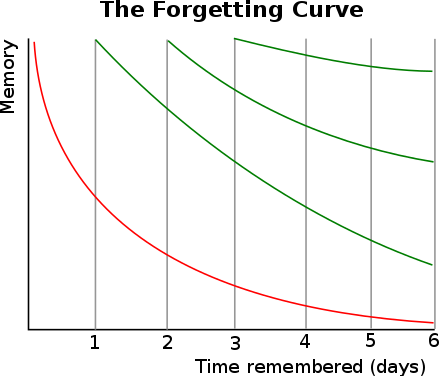
\includegraphics[width=0.4\textwidth]{images/vergessenskurve.png}
    \caption{ebbinghaussche Vergessenskurve \protect}
    \label{fig:curve}
\end{figure}

Auffällig an dem Modell ist die exponentiell ähnliche Abnahmen des erlangten Wissens. Die rote Kurve beschreibt den Anteil an gemerktem Wissen ohne eine weitere Wiederholung. Ebbinghaus hält fest, dass er nach 20 Minuten nur noch in der Lage war, 60\% richtig wiederzugeben. Nach einer Stunde waren es noch 45\%. Einen Tag und sechs Tage danach lag das gemerkte Wissen nur noch bei 34\% bzw. 23\%. Über einen langen Zeitraum festigen sich nur rund 15\% des geübten Wissens. Wird der Lernprozess durch Wiederholungen (grüne Graphen) ergänzt, festigt sich das Thema mit der Zeit. Die Kurve flacht schneller ab und ist generell weniger steil \cite{Wiki:Vergessenskurve}.

Kritisiert wird das Modell von Forschern in Hinsicht auf das Selbstexperiment \cite{Wiki:Vergessenskurve}. Es wird hinterfragt, wie geeignet ein Selbstexperiment zur Erfassung des Erinnerungsvermögens ist und inwiefern äußere Ereignisse Einfluss auf das Ergebnis hatten. Das Ebbinghaus sinnlose Silbenreihen genutzt hat, wird ebenfalls kritisiert, da Neurologie und Gehirnforschung gezeigt haben, dass persönlich bedeutsame Themen anderen Vergessenskurven unterliegen \cite{Wiki:Vergessenskurve}. Damit wurde bewiesen, dass Vergessen abhängig vom zu verinnerlichen Wissen ist, was in den Selbstversuchen nicht berücksichtigt wurde. C. Michel und F. Novak haben in neuen Studien \cite{Wiki:Vergessenskurve} diese Komponente berücksichtigt und den Anteil an vergessenem Wissen nach 5 Tagen und 30 Tagen festgehalten. Am wenigsten wurden Prinzipien und Gesetzmäßigkeiten vergessen (1\% bzw. 5\% wurden vergessen). Gedichte konnten zu 75\% bzw. 50\% nach verstrichener Zeit wiedergegeben werden. 53\% bzw. 60\% von den zuvor erlernten Prosa wurden vergessen. Die von Ebbinghaus genutzten sinnlosen Silbenreihen werden am schnellsten Vergessen. Nach der Zeit konnten lediglich 22\% bzw. 20\% richtig wiedergegeben werden \cite{Wiki:Vergessenskurve}

Für die Applikation ist das Modell von Ebbinghaus trotz der Kritik eine gute Orientierung, weil Schüler ein Spektrum an unterschiedlichen Dingen lernen müssen. Es lohnt sich nicht, für alle Möglichkeiten unterschiedliche Vergessenskurven als Grundlage zu nehmen. Außerdem sind die Fälle für ein Programm schwer zu unterscheiden, weshalb von dem schlechtesten Fall ausgegangen werden sollte.

\subsection{Konzept von Spaced Repetition}
Nach der Entdeckung der ebbinghausschen Vergessenskurve folgten Ansätze für ein darauf basierendes Lernverfahren. Mit \textit{Spaced Repetition} sollte gegen das schnell abfallende Wissen gewirkt werden, indem die eingängliche Wiederholung mit weiteren unterstützt wird. Dabei wird der Abstand der nachfolgenden Wiederholungen regelmäßig erhöht, um sich an die sinkende Verfallsrate von gefestigten Wissen anzupassen. 

Die anfängliche Idee war es, Karteikarten in Boxen zu kategorisieren. Die Boxen wurden von eins bis fünf mit Zahlen, welchen den Fortschritt widerspiegeln, durchnummeriert. In der ersten Box sind die Karten, welche der Schüler am schlechtesten beherrscht. Wenn die Karteikarte erfolgreich wiedergegeben wurde, dann wird die Karte in die nächst höhere Box gelegt. Eine Karte aus der Box eins würde dann in die Box 2 gelegt werden. Wenn eine Karte nicht wiedergegeben werden kann, dann wird diese egal wo sie vorher war, wieder in die Box eins gelegt. Beim lernen werden die Karten in der ersten Box priorisiert, um auf die Schwächen zu fokussieren.

\textit{Cramming}, eine zur \textit{Spaced Repetition} adverse Lernmethode, in welcher über einen kurzen Zeitraum Wissen angeeignet wird, ist bei vielen Schülern die standard Lerntechnik. Die damit verbundenen negativen Aspekte sind von der Hand zu weisen. Da bei dieser Methode nötige Wiederholungen fehlen, steht angeeignetes Wissen nur temporär zur Verfügung, was mit den Erkenntnissen der ebbinghausschen Vergessenskurve übereinstimmt. Das ist besonders kritisch, wenn andere Themen darauf aufbauen. Wegen dieser Gründe, sollte von \textit{Cramming} abgesehen werden und auf \textit{Spaced Repetition} zurückgegriffen werden.

\subsection{Ergebnisse von Studien}
Es liegen diverse Studien vor, welche die Effektivität von \textit{Spaced Repetiton} analysieren und bestätigen \cite{PNAS:Synaptic}\cite{RD:SpacedRepetition}. Dabei fächern sich die Beweismethoden auf verschiedene Bereiche, darunter Gehirnscans, womit die Stärke von synaptischen Verbindungen analysiert wird und experimentelle Studien, in welchen mit Probanden diverse Lernmethoden verglichen werden.

A. Voice und A. Stirton haben in \cite{RD:SpacedRepetition} eine Software für die Probanden entwickelt, die auf dem \textit{Spaced Repetition} Prinzip aufbaut, und die Auswirkungen auf das Prüfungsergebnis analysiert. Dafür wurde je einer Gruppe von Thermodynamik-Studenten die Software direkt nach Start, nach einem Sechstel und nach einem Drittel des Jahres vorgestellt. Dazu wurde mit irregulären Erinnerungen über das Jahr verteilt auf die Anwendung aufmerksam gemacht. Neben der Applikation konnten die Schüler lernen, wie sie wollten. Am Ende des Lehrjahres folgte eine Prüfung des Lernstands. Anschließend wurden die Testergebnisse verglichen. Während in dem ersten Jahr kein signifikant besseres Ergebnis der App-Nutzer gegenüber den nicht App-Nutzer erkennbar ist, kristallisiert sich in den Ergebnissen der darauf folgenden Jahrgänge eine signifikante Verbesserung der Lernleistung heraus. Ergänzend zur Prüfung folgte nach den Ferien ein unangekündigter Test, mit welchen das Langzeitpotenzial getestet wurde. Generell lagen schlechtere Ergebnisse der Schüler nach den Ferien vor, was mit dem Prinzip der ebbinghausschen Vergessenskurve übereinstimmt. Im Vergleich zwischen Nutzern und Nichtnutzern zeigten die Nutzer ein signifikant höheres Ergebnis, was das Langzeitpotenzial von \textit{Spaced Repetition} bestätigt.

In \cite{PNAS:Synaptic} untersuchen E. A. Kramár et al. die Stärke der Synapsenverbindungen in Hinblick auf das Langzeitpotenzial. Dafür wurden Synapsen eines Rattenhippocampus angeregt. Nach regelmäßigen Abständen wird die ursprüngliche Verbindung neu stimuliert. Dabei ging eine Steigerung Potenzierung nach 60 und 90 Minuten hervor. Eine erneute Stimulierung nach 10 oder 20 Minuten hat eine vergleichsweise minimale Steigerung. Des Weiteren hat die Studie festgestellt, dass eine dritte und vierte Stimulierung nach jeweiligen 60 Minuten kaum bis keine Auswirkungen auf die Langzeitpotenzierung hat, was einen steigenden Wiederholungsintervall impliziert. Ein Anstieg an Synapsen konnte von den Forschern ebenfalls nachgewiesen werden.

\section{Dart und Flutter}
\label{dart_flutter}
Dart ist eine von Google entwickelte Programmiersprache, welche auf Anwendungsentwicklung fokussiert ist, aber auch für Server genutzt werden kann. Anwendungen, die mit Dart programmiert werden, können Mobile Applikationen, Webseiten oder Desktop-Anwendungen sein. Dart implementiert viele herkömmliche Programmierpraktiken, wie Objektorientierung, Klassen und automatisierter Garbage Collection. Dart erschien erstmals am 10 Oktober 2011.

Das Beispiel \ref{lst:beispiel} zeigt rudimentäre Elemente von Dart. Es lassen sich viele Gleichheiten mit Programmiersprachen wie C\# und Java erkennen. Der Einstiegspunkt in das Programm ist in Dart ein wenig leichter gestaltet. Auffällig ist die für Dart typische dynamische Variablen Deklaration mit \texttt{final} für Variablen, welche einen konstanten Wert beibehalten. Ebenfalls zeigt die Zeile, dass bei Klasseninitialiserungen \textit{named parameter} angegeben werden. Jedoch ist dies nur der Fall, wenn in den Parameterklammern des Konstruktors geschweifte Klammern angegeben werden. Damit werden die Paramter zu optionalen namentlichen Parametern und müssen nicht angegeben werden. Das Schlüsselwort \texttt{required} wirkt gegensätzlich, sodass der Parameter doch angegeben werden muss. In Kombination aus geschweiften Klammern und dem Aufruf von Attributen, wird eine verkürzte Schreibweise für anfängliche Wertzuweisungen ermöglicht. In dem Beispiel \ref{lst:beispiel} wird das Attribut in den Konstrukt der Klasse \texttt{Zaehler} direkt mit dem Wert 100 initialisiert.

Die dynamische Syntax spiegelt sich auch in Dart-Methoden wieder. Rückgabewerte sind optional und es muss kein Schlüsselwort für Methoden angegeben werden, wie es in Python der Fall ist. Der Name und die Parameterklammern reichen aus. Die Rückgabe eines Wertes lässt sich auf zwei Weisen erreichen. Die herkömmliche Version lässt sich auch in C\# und Java finden. Dafür wird in dem Methodenkörper mit \texttt{return} ein Wert wiedergeben. Dafür hat Dart ebenfalls eine verkürzte Schreibweise. Mit \texttt{=>} wird der Ausdruck \texttt{{ return expr; }} abgekürzt. Damit sind geschweifte Klammern nicht mehr von Nöten und der Wert, welche aus der Zeile hervorgeht, wird von der Methode ausgegeben. Hierbei ist zu beachten, dass die verkürzte Schreibweise nur dann benutzt werden darf, wenn nur eine Zeile folgt. Für mehrere Zeilen muss auf die gewohnte Schreibweise zurückgegriffen werden. Dafür ist es genauso möglich nichts zurückzugeben, somit kann \texttt{=>} auch für \texttt{void}-Methoden genutzt werden.

\begin{lstlisting}[caption={Dart Beispiel},captionpos=b,label={lst:beispiel},numbers=left,frame=none,escapechar=|]
void main() {
  final b = Zaehler(amount: 100);
  b.alleFuenfAusgeben();
}

class Zaehler {
  int amount;

  Zaehler({required this.amount});

  alleFuenfAusgeben() {
    for (int i = 0; i < amount; i++) {
      if (fuenffach(i)) {
        print('hello ${i + 1}');
      }
    }
  }

  fuenffach(int zahl) => (zahl + 1) % 5 == 0;
}
\end{lstlisting}

Am 4 Dezember, 2018 wurde das \textit{open-source software development kit} Flutter in seiner ersten stabilen Version von Google veröffentlicht. Flutter umfasst ein komplettes \textit{Framwork} mit vorgefertigten \textit{Widgets} und \textit{Tools}. Eine mit Flutter programmierte Anwendung besteht aus vielen Widgets, welche auch wieder \textit{Widgets} beinhalten können. \textit{Buttons} oder \textit{Textfields} beispielsweise auch \textit{Widgets}. Kompiliert wird die Anwendung zu nativen \textit{Code}, entweder durch \textit{ahead-of-time} oder \textit{just-in-time} Kompilation. Bis zu Flutter 2 waren Programme für Android und IOS verfügbar. Mit der neuen Version vom 3 März 2021 wurden die Zielplattformen um Web, Windows, Linux und macOS ergänzt.

Trotz, dass Flutter relativ neu ist, haben Unternehmen unterschiedlichster Branchen Flutter adaptiert \cite{Flutter:Usage}. Da es ein Produkt aus dem Hause Google ist, wird es dort auch für Applikationen wie \textit{Google Pay} genutzt. Ein weiterer Vertreter des amerikanischen Markts ist Ebay, welcher für ebay motors eine Ebay ähnliche Applikation für Auto bezogene Themen mit Flutter entwickelt hat. Das Anwendungsentwicklungsteam des deutschen Autoherstellers BMW vertraut auf Flutter für die Autos begleitende Applikation. Flutter wird auch von asiatischen Unternehmen genutzt. Die Tech-Unternehmen Alibaba, Tencent, ByteDance und Toyota bedienen sich ebenfalls an dem Flutter Framework. Die Entwickler der aufgelisteten Unternehmen sprechen laut \cite{Flutter:Usage} von Leistungs- und Effektivitätssteigerungen. 

    \chapter{Konzeptionierung}
In diesem Kapitel wird das Konzept für die Applikation aufgestellt, indem die Anforderungen definiert werden und die darauf basierenden Features der Anwendung diskutiert werden. Ergänzend werden die nötigen Backend- und Serverfunktionen erötert, um die Features zu verwirklichen.
% -------------------------------------------
% Anforderungen
% -------------------------------------------
\section{Anforderungen}
\label{section:rahmenbedingungen}
Im Folgenden werden die Rahmenbedingungen und Anforderung an die Applikation im Hinblick auf die tägliche Nutzung der primären Zielgruppe Schüler definiert. Wie schon in Kapitel \ref{einleitung} erörtert, ist das Hauptziel der Anwendung, Schüler so gut wie möglich beim Lernprozess zu unterstützten. In Betrachtung dieses Ziels werden drei Anforderungen an die Applikation erkennbar:
\begin{description}
\item[1. Verständlichkeit]
Dadurch, dass in der Schule viele unterschiedliche Kompetenzstufen zusammen kommen, muss eine solche Anwendung nicht nur erfahrene Nutzer ansprechen, sondern intuitiv auch von weniger erfahrenen Benutzern bedienbar sein. Während Nutzer Prozesse aus dem Kontext mithilfe logischer Schlussfolgerung und übergreifenden Richtlinien ableiten können, fehlt diese Intuition den unerfahrenen. Somit ist es wichtig, die Applikation so einfach wie möglich zu gestalten. Das minimiert die Gefahr, dass kein Schüler durch technisches Ungeschick Nachteile erleidet. Unterstützt wird die benutzerfreundliche Oberfläche durch eine detaillierte Anwendungshilfe.
\item[2. Verfügbarkeit]
Ein offensichtlicher, dennoch oft vergessener Punkt ist, dass alle Schüler das Tool verwenden können sollen. Dabei ist die entscheidende Frage die Wahl der Plattform, da finanziell schwache Familien häufig weniger technische Hilfsmittel zur Verfügung stehen. Daraus ergibt sich die Herausforderung, auch diesen Kindern einen Zugriff auf optimale Lernmethoden und Umgebungen zu gewährleisten. Unter diesen Punkt fällt ebenfalls, dass die Applikation so günstig wie möglich sein sollte, damit auch finanziell schwache Anwender von den Vorteilen der Anwendung profitieren können.
\item[3. Zentrale Lernstoffverwaltung]
Als Letztes ist eine gleiche Informationsgrundlage für einen gleichberechtigten Lernprozess von Nöten. Mithilfe einer zentralen Sammlung des Lehrstoffs werden unterschiedliche Datenlagen ausgeschlossen. Eine solche Sammlung sollte durch Lehrkräfte verwaltet werden, um Unterrichtsmaterialien, Vokabellisten und weiteren Lernstoff einheitlich für Schüler bereitstellen zu können.
\end{description}

% -------------------------------------------
% Funktionen
% -------------------------------------------

\section{Funktionen}
In diesem Abschnitt werden die einzelnen Funktionen der Applikation erörtert. Dabei wird der Fokus auf Begründungen und Gedankengänge gelegt, welche im Kapitel \ref{section:programmierung} implementiert werden. Die Funktionen der Applikation sind unter besonderer Berücksichtigung der im Abschnitt \ref{section:rahmenbedingungen} aufgestellten Rahmenbedingungen entworfen worden.

\subsection{Dateimanagement}
Damit der Nutzer einen Überblick über alle Karteikarten behält, werden diese in einem System ähnlich einer Ordnerstruktur organisiert. Um eine passende Repräsentation zu wählen, wurde für die Speichermöglichkeiten ein typisches Beispiel für Schüler reproduziert. Die gespeicherten Karten lassen sich in erster Ordnung in verschiedene Fächer teilen. Karteikarten für Mathematik, Englisch und Deutsch sollten sichtlich voneinander unterscheidbar sein. Jedes Fach kann zudem noch in einzelne Themen unterteilt werden. Am Beispiel Mathematik könnten mögliche Themen Algebra und Analysis sein. Diese Themen lassen sich in weitere Unterthemen einteilen, wie Integralrechnung, Extremstellenberechnung und andere. 

Folglich sollten die Ordner, welche die Themen repräsentieren, unbestimmt tief reichen. Dafür wurde grundlegend auf ein gleiches System wie jede herkömmliche Ordnerstruktur zurückgegriffen. Die Abbildung \ref{fig:appdatabase} zeigt, dass die Ordner der Anwendung in einer SQL-Datenbank gespeichert werden. Die Tabelle \texttt{folder} hat 7 Attribute, wobei 3 für das Speichern relevant sind. Der Index eines Eintrags ist ein eindeutiger Wert und ein Ordner kann damit bestimmt werden. Das Attribut \texttt{name} trägt eine lesbare Bezeichnung des Ordners, die vom Nutzer vergeben werden kann. Der Wert muss nicht eindeutig sein und kann beispielsweise Mathematik, Englisch, Algebra oder Analysis sein. Als Letztes bestimmt \texttt{root}, ob ein Ordner Unterordner hat, indem jeder Ordner speichert, welcher der übergeordnete Ordner ist. Durch diese Art der Konstruktion können durch eine einfach SQL-Abfrage mit Filter auf dem Feld \texttt{root} alle Unterordner für einen spezifischen Ordner gefunden werden. Da es sich hierbei um eine 1:n-Beziehung handelt, kann ein Ordner eine beliebige Zahl Unterordner enthalten.

\begin{figure}[ht!]
  \centering
  \begin{minipage}[b]{0.4\textwidth}
    \includegraphics[width=\textwidth]{images/add_before.png}
    \caption{Ordneransicht, bevor der \textit{FAB} zum Hinzufügen gedrückt wurde}
    \label{add_before}
  \end{minipage}
  \hfill
  \begin{minipage}[b]{0.4\textwidth}
    \includegraphics[width=\textwidth]{images/add_after.png}
    \caption{Ordneransicht, nachdem der \textit{FAB} zum Hinzufügen gedrückt wurde}
  \end{minipage}
\end{figure}

Auf jeder Ansicht, außer der Suche und des Kartenlernen, ist es für den Nutzer möglich, Karten und Ordner zu erstellen. Dafür wird ein \textit{Floating Action Button} (\textit{FAB}) in der rechten unteren Ecke angezeigt. Wenn der \textit{FAB} gedrückt wird, dann wird um zwei weitere Optionen ergänzt. Mit den neuen Optionen lassen sich Ordner und Karten erstellen. Für einen Ordner muss ein Name angegeben werden. Optional sind Pfad und ob der Ordner öffentlich ist. Standardmäßig wird für den Pfad der Ordner ausgewählt, welcher ausgewählt war, als der Ordner erstellt wurde. Wenn ein Ordner in einem Ordner mit Karten erstellt wird, dann werden die Karten in einen Subordner \textit{Karten} umsortiert.

Gegensätzlich Ordner löschen geht über die Einstellung der Ordner. Entweder kann auf einen Ordner lange gehalten werden oder in einem Ordner auf das Zahnrad, welches Einstellungen weitgreifend darstellt, geklickt werden, um die Einstellung zu öffnen. In den Einstellungen kann der Ordner nicht nur gelöscht werden, sondern auch der Name geändert, der Pfad geändert und der Ordner aufgelöst werden. Beim Ändern des Pfads wird die zuvor erläuterte \texttt{root} auf einen neuen Wert geändert. Während beim Löschen der komplette Inhalt des Ordners gelöscht wird, wird beim Auflösen eines Ordners der Inhalt auf den Überordner übertragen. 

Beim Erstellen einer Karte, werden Vorderseite und Rückseite gefordert. Die Vorderseite ist der Wert, welcher während des Lernprozesses jeder Zeit angezeigt wird. Optional können wieder Pfad und Zugangsberechtigung definiert werden. Der Pfad wird durch der \texttt{root} Feld der Karte gespeichert. Über die Referenz zum Ordner, kann der Inhalt des Ordners mit einer SQL-Abfrage bestimmt und angezeigt werden. Dafür muss der \texttt{index} der Ordners in der \texttt{card} Tabelle gesucht werden und alle Treffer sind Karten.

Für eine erweiterte Struktur können Karteikarten und Ordner nicht zusammen erscheinen. Das bedeutet, wenn ein Ordner Unterordner hat, kann dieser keine Karten mehr enthalten. Um das zu gewährleisten wird nicht nur das Hinzufügen blockiert, sondern auch das Äuflösen von einem Ordner mit Karteikarten. Die Idee dahinter ist es Thema und Inhalt sichtlich und verständlich zu trennen.

% ------------ Lernen von Karten ------------
\subsection{Lernen von Karten}
In jeder Ansicht wird dem Nutzer ein großer, grüner \texttt{Button} präsentiert. Bei Drücken des \texttt{Buttons}, wird eine neue Ansicht geladen. In dieser Ansicht werden alle Karten präsentiert, welche in den Unterordnern vorhanden sind. Die Reihenfolge der Karten basiert dabei, auf dem vorher thematisierten Prinzip von \textit{Spaced Repetition}. Für jede Karte wird in der Datenbank eine Zahl gespeichert. Karten, die basierend auf der bisherigen Lernleistung als unsicher eingestuft werden, werden dem Nutzer als erstes zur Wiederholung angezeigt. Um die Frustration des Nutzers gering zu halten, werden zwischen die unsicheren Karten, manchmal leichtere, schon bekannte Karten gemischt. Das basiert auf dem Prinzip, dass die Motivation von Menschen am höchsten ist, wenn wir weder vor einem, für unseren Wissensstand, zu schweren oder leichtem Problem stehen \cite{AtomicHabits}.

Sobald der Nutzer eine Karte eingesehen hat, stehen ihm zwei Möglichkeiten zur Verfügung, um sein Verständnis zu überprüfen. Wenn nach links gewischt wird, bedeutet das, dass der Nutzer die Karte nicht konnte und damit wird die Zahl der Karte wieder auf 0 reduziert. In dem Fall, dass die Karte nach rechts geschoben wird, wird dem System gesagt, dass der Nutzer die Karte auswendig konnte. Danach wägt das System die neue Zahl für die Karte mit einem Algorithmus ab. Dieser setzt sich zusammen aus:

\begin{description}
\item[1. Betrachtungsdauer der Vorderseite]
Eine kurze Zeit bedeutet, dass der Nutzer sofort wusste, was auf der Rückseite steht oder im gegensätzlichen Fall, direkt wusste, dass er es nicht weiß. Bei einer relativ langen Zeit kann davon ausgegangen werden, dass der Nutzer lange brauchte um sich die Erinnerung an die Rückseite ins Gedächtnis zu rufen.
\item[2. Betrachtungsdauer der Lösung]
Ein kurzes betrachten der Rückseite legt nahe, dass die Karte bekannt war. Die Karte war weitestgehend bekannt, wurde aber sicherheitshalber mehrmals gelesen oder ein kleiner Fehler ist unterlaufen, welcher für den Gesamtkontext von marginaler Auswirkung war, wenn die Rückseite länger angeschaut wird.
\item[3. Die Länge des Inhalts der Vorderseite.]
Die im ersten Punkt gemessene Zeit der Vorderseite muss in Relation zur Länge der Vorderseite gebracht werden. So lässt sich der Inhalt einer Kartenvorderseite schneller lesen und bearbeiten, wenn dieser nur aus einem einzigen Wort besteht. Enthält die Karte jedoch mehrere Sätze, so steigt die Bearbeitungszeit mindestens linear an.
\item[4. Die Länge des Inhalts der Rückseite.]
spielt nicht nur eine Rolle für den Punkt 2 basierend auf dem in Punkt 3 erklärten Prinzip, sondern ist auch wichtig für Punkt 1, da ein kurzer Inhalt schneller wiedergegeben werden kann als ein langer.
\end{description}

Anhand dieser Gesichtspunkte ist das System in der Lage abzuwägen, wie gut der Nutzer die Karte konnte. Folgende Bedingungen konzentrieren sich auf den Fall, dass der Nutzer nach rechts wischt. Wenn die Zeit, mit welcher der Nutzer sich die Vorderseite angeguckt hat, relativ zur Länge der Vorderseite kurz ist und die Rückseite nur kurz angeguckt wurde oder gar nicht, kann davon ausgegangen werden, dass der Nutzer die Karte gut beherrscht. Der ermittelte Wert ist damit sehr hoch. Der Nutzer beherrscht die Karte schlecht, wenn die Dauer der Vorderseite, wie oben geschildert, ebenfalls kurz ausfällt, aber die Rückseite dafür relativ Lange angeschaut wird. Es lässt sich vermuten, dass versehentlich nach rechts gewischt wurde oder ein Fehler unterlaufen ist, welcher aber ignoriert wurde. Im mittleren Fall, dauert die Vorderseite länger, aber die Rückseite ist vergleichsweise schnell. In dieser Möglichkeit, hat der Nutzer etwas länger braucht um auf die Lösung zu kommen, hatte sie aber richtig. Deswegen ist die Wertung mittel.

% -------------- Statistiken ----------------
\subsection{Statistiken}
Nach \cite{AtomicHabits} wirkt direkte Visualisierung des Fortschritts motivierend auf den Menschen. Dazu und um die Nutzererfahrung zu verbessern, indem eine optimale Lernzeit ermittelt wird, werden Statistiken angezeigt. Diese wurden mithilfe von Sessions verwirklicht. Beim Start eines Lernabschnitts wird eine Session gestartet. Für jede Session wird das Datum, die Start- und Endzeit, die Nummer des Ordners und die Anzahl an falschen und richtigen Karten gespeichert. Eine Session endet entweder damit, dass die Ansicht verlassen, die Applikation geschlossen wird oder länger als eine Minute im Hintergrund verweilt.

Mit den gesammelten Daten werden in der Statistiken-Ansicht detailliertere Informationen über die Nutzungsgewohnheiten anschaulich aufbereitet. In Abbildung \ref{fig:statistics} wird die Ansicht der Statistik dargestellt. In der ersten Reihe werden alle Karten im Ordner und die komplette gelernte Zeit angezeigt. Darunter folgt eine umfangreiche Ansicht der gelernten, ungelernten und neuen Karten. Es lässt sich der Zeitraum auswählen, welcher ein Jahr, Monat, Woche oder Tag sein kann. Für den Zeitraum lassen sich detaillierte Informationen abrufen, indem mit dem Finger über den Graphen gegangen wird. Für die Stelle, an der der Finger ist, wird die genau Anzahl an jeweiligen Karten angezeigt. Nach dem Graphen folgen zwei Ansichten für die durchschnittliche Nutzeraktivität. In der ersten Ansicht wird der Zeitraum angezeigt, in welchem der Nutzer am meisten lernt. Die zweite Statistik zeigt die Zeiträume, in welchen der Nutzer am effektivsten ist. Ermittelt wird das, indem die Anzahl der richtigen und falschen Karten in Relation zueinander und der kompletten Anzahl an gelernten Karten errechnet wird und der daraus resultierende Durchschnitt wird in die Ansicht eingefügt. Der Wert wird für jede Uhrzeit ermittelt und ermöglicht so einen guten Überblick darüber, wann am effektivsten gelernt wurde. Abgeschlossen wird die Anzeige der Statistik mit einem zusammenfassenden Satz, welcher eine optimale Lernzeit aus den vorliegenden Daten ermittelt. Dafür werden Effektivität und Zeit zusammengeführt und der Zeitraum mit den höchsten Werten ermittelt. Bei der Zusammenführung wird die Effektivität mehr gewichtet. Im Optimalfall kann für die Nutzer eine passende Lernzeit ermittelt werden, welche einerseits in den Zeitplan der Nutzer passt und andererseits die Effektivität der Lernzeit möglichst hochhält.

\begin{figure}[ht!]
    \centering
    \includegraphics[width=0.3\textwidth]{images/statistiken.png}
    \caption{Detailliert Ansicht der Nutzeraktivität}
    \label{fig:statistics}
\end{figure}

Darüber hinaus wird in jedem Ordner eine vereinfachte Ansicht für die gelernten, ungelernten und neuen Karten angezeigt, wie in Abbildung \ref{add_before} dargestellt. In dieser stehen keine detaillierten Informationen zur Verfügung und der Zeitraum ist ebenfalls auf den größtmöglichen festgelegt. Angezeigt wird die vereinfachte Ansicht, um als Knopf zur detaillierten Ansicht zu fungieren und den von \cite{AtomicHabits} erläuterten Effekt zu stärken, indem nicht in die detaillierte Ansicht gewechselt werden muss, um den Fortschritt anzusehen.

% ------------------ Kurse ------------------
\subsection{Kurse}
Mit dem Fokus auf eine schulähnliche Umgebung, dürfen Klassen bzw. Kurse nicht fehlen. Ein Kurs funktioniert in der Anwendung genauso wie in der Schule. Ein Nutzer kann einen Kurs erstellen und verwalten. Das bezieht sich auf die Mitglieder und die Inhalte, beide können nach Belieben wieder entfernt werden. Der große Vorteil an Kursen ist, dass mit ihnen Inhalte einfach geteilt werden können. In den Einstellungen kann das Teilen auch für Nutzer freigegeben werden, entweder mit oder ohne Überprüfung des Verwalters.

Finden lässt sich der Inhalt der Gruppen in einem neuen Ordner namens \textit{Gruppen} auf der Startansicht. Jede Gruppe hat ihren eigenen Unterordner und die darin enthaltenen Inhalte sind die mit der Gruppe geteilten Ordner und Karteikarten. Persönliche Änderungen können, ohne jeglichen Effekt für die anderen Nutzer, vorgenommen werden. Die eigenen Änderungen werden durch zentrale Änderungen an den jeweiligen Karteikarten überschrieben.

Um einen Kurs beizutreten, kann ein QR-Code innerhalb der Anwendung eingescannt werden. Der Scanner findet sich in der Suchleiste. Sobald der QR-Code eingescannt wurde, wird der Nutzer dem System mitgeteilt und dem Kurs hinzugefügt. Die Inhalte des Kurses werden dann auf das Gerät heruntergeladen.

Anwendungsfälle für Kurse sind Zusammenfassungen der Unterrichtsstunden, die einzelnen Themen in Karteikarten zusammengefasst oder für Klausuren, noch einmal jedes Thema verständlich summiert. Mit diesen Ordnern kann für die Klausur gelernt werden. Über den Verlauf des Jahres sollten die Unterrichtsstunden wiederholt werden und zur Vorbereitung auf die Klausur wird auf die Ordner mit den Klausurthemen gewechselt. So kann über das Jahr der Inhalt gefestigt werden und die Themen der Klausurvorbereiten sollten so leichter fallen.

% ------------ Teilen von Ordnern -----------
\subsection{Öffentliche Ordner}
Online Ordner funktionieren ähnlich wie Kurse. Die beiden unterscheiden sich lediglich in der adressierten Zielgruppe. Kurse lassen sich nicht in der Suche finden, da diese privat gehalten und begleitend zum Unterricht geführt werden sollen. Die Online Ordner wiederum sind als Ordner von anderen für andere angesehen. So können bilinguale Nutzer einen Ordner erstellen, mit dem Interessierte Sprachen lernen können. Damit soll ermöglicht werden, dass Themen von Experten aufbereitet und der breiten Masse zum eigenständigen Lernen zur Verfügung gestellt werden.

Verwirklicht wird das, indem die Ordner in ihren jeweiligen Einstellungen eine Option zum Veröffentlichen haben. Sobald diese aktiviert wird, sind die Daten für jeden zugänglich. Gefunden werden die Ordner mit der Suchleiste, über den Namen des Ordners. Die Ordner können bei Interesse heruntergeladen und bearbeitet werden. Dabei greift das gleiche Prinzip wie bei Gruppen. Änderungen sind nur temporär und sobald die Karteikarte mit den Änderungen aktualisiert wird, werden die alten Werte überschrieben. Das damit verbunden Potential für mögliche Weiterentwicklung in diesem Bereich wird im Fazit unter Abschnitt \ref{weiteresvorgehen} noch einmal aufgegriffen.

% -------------------------------------------
% Entwurf des Backends
% -------------------------------------------

\section{Entwurf des Backends}

% ------ Clientside ------
\subsection{Clientside}
\begin{figure}[ht!]
    \centering
    \includegraphics[width=1\textwidth]{images/app_datenbank.png}
    \caption{Datenbank der Anwendung}
    \label{fig:appdatabase}
\end{figure}

% ------ Serverside ------
\subsection{Serverside}
Das Backend des Servers besteht aus der Programmiersprache Python und dem \textit{Relation Database Management System} MySQL. Python bildet die Logik des Servers und MySQL ist die SQL-Schnittstelle zur Datenbank. Wenn eine Abfrage an den Server gestellt wird, arbeiten beiden zusammen, um eine \textit{Response} an den Nutzer zu schicken.

% das hier ist alles out of mind geschrieben -> muss noch mit echten Daten gefüttert werden.
Python ist eine von Guido van Rossum entwickelte high-level Programmiersprache, welche einen hohen Wert auf einfach Syntax legt. Python ist mittlerweile zu der meist genutzten Programmiersprache der Welt geworden. Am meisten wird sie für Scatch-Programming, Data-Analytics und AI-Programming genutzt. MySQL ist eine SQL-Programmiersprache, welche ähnlich wie die im Unterricht thematisierte Programmiersprache SQLite funktioniert. Der zentrale Unterschied der beiden ist, dass MySQL schneller ist und mehr Features hat. Dafür wird für SQLite kein Server gebraucht.



Für den Server wurde auf den Anbieter Linode zurückgegriffen 
Linode erklären
Datenbank erklären

Einleitung
Bild von der Datenbank
Datenbank erklären und Gedanken erläutern, wieso ich mich für diese Tabellen und Darstellungsmöglichkeiten entschieden habe.

% ------ Datenaustausch ------
\subsection{Datenaustausch}

Informationen werden in Form von \textit{https-requests} an den Server geschickt. Über diese Weise sind die übermittelten Informationen Standardmäßig verschlüssel. Formatiert sind sind die Informationen in einem JSON String. Die Informationen werden aus dem übergebenen JSON String gefiltert und verarbeitet.

Die Applikation wird über Änderungen informiert, indem der Server registriert, ob eine neue Version hochgeladen wird. Das Änderungsdatum wird mit in die Datenbank eingetragen. Die Applikation ruft vom Server alle Änderungen der verlinkten Boards ab, sobald diese aufgerufen wird. Die Response vom Server an die Applikation ist ein Datenpacket mit allen neu Hinzugefügten Elementen. Diese können als einfach Tabelle angefügt werden, da durch das vorher erstellte System, Änderungen einfach anzuwenden sind.

%QT Hier einen typsichen Datenaustausch darstellen

%QT Hier ein typisches Update eines Ordners darstellen

% -------------------------------------------
% Sicherheit
% -------------------------------------------

\section{Sicherheit}
In Deutschland wird ein hohes Augenmerk auf die Sicherheit von Nutzerdaten gelegt. Wer in Deutschland eine Applikation mit Nutzerdatenverwaltung veröffentlich möchten, muss sich an die Datenschutz-Verordnung (DSGVO) halten. Diese bezieht sich auf Daten die automatisiert und nicht automatisiert verarbeitet werden. Die Grundsätze der DSGVO werden im Artikel 5 definiert.
\begin{description}
\item[1. Rechtmäßigkeit, Verarbeitung nach Treu und Glauben, Transparenz]
Die Daten müssen auf rechtmäßige Weise und für betroffene Personen nachvollziehbar verarbeitet werden.
\item[2. Zweckbindung]
Daten dürfen nur für festgelegte, eindeutige und legitime Zwecke gespeichert werden.
\item[3. Datenminimierung]
Das Maß der gespeicherten Daten sollte sich auf die für den Zweck nötigen Daten beschränken
\item[4. Richtigkeit]
Daten müssen sachlich richtig und auf den neusten Stand sein. Fehler müssen sofort gelöscht oder behoben werden.
\item[5. Speicherbegrenzung]
Daten, mit welchen auf Personen zurück geschlossen werden kann, dürfen nur solange gespeichert werden, wie sie für den Zweck gebraucht werden.
\item[6. Integrität und Vertraulichkeit]
Es muss eine angemessene Sicherheit für das speichern der Daten herrschen. Das beinhaltet den Schutz vor unbefugter und unrechtmäßiger Verarbeitung.
\end{description}

\subsection{Salt und Secret Salt}
Um sich bei dem Programm zu authentifizieren, wird von dem Nutzer eine Kombination aus Passwort und Nutzername genutzt. Diese beiden Informationen werden an den Server geschickt, welcher überprüft ob Nutzername und Passwort richtig angegeben worden sind. Das wird gemacht, indem Nutzername und Passwort mit den Einträgen in der Datenbank abgeglichen werden. Einher geht, dass wenn die Datenbank von Unbefugten kopiert wird, alle Nutzernamen mit ihren jeweiligen Passwörtern einsehbar sind. Damit können sich die Angreifer als andere Person ausgeben. Folglich, ist Speichern von Passwörtern in Klartext auf Servern grob fahrlässig.

Um diesem Fall entgegen zu wirken werden Passwort in modernen Systemen verschlüsselt. Ein häufig verwendetes Verfahren ist der SHA-256 Algorithmus. Das in 2001 veröffentliche und von der \textit{National Security Agency} entwickelte Verschlüsselungsverfahren basiert auf dem \textit{Merkles Meta-Verfahren}. Eine mit diesem Verfahren verschlüsselte Zeichenkette ergibt jedes mal das gleiche Ergebnis und es fast unmöglich die Zeichenkette aus dem Verfahren rückzuschließen. Ein weiterer Vorteil, ist das kleine Abweichen einen großen Einfluss auf das Ergebnis haben, wie an folgenden Beispielen erkennbar.

\textbf{QT BEISPIEL!} \break
Zeichenfolge 1: password \break
Zeichenfolge 2: passw0rd \break\par

SHA-256 Output 1: \break 5e884898da28047151d0e56f8dc6292773603d0d6aabbdd62a11ef721d1542d8 \break
SHA-256 Output 2: \break 8f0e2f76e22b43e2855189877e7dc1e1e7d98c226c95db247cd1d547928334a9

Zeichenfolge 1 und Zeichenfolge 2 unterscheiden sich in einem Zeichen. Das Resultat des Ergebnisses ähnelt sich jedoch nur in 3 Zeichen. Mithilfe der beiden SHA Ergebnissen, ist es nicht möglich einen Zusammenhang zwischen den Passwörtern zu erstellen.

Dadurch, dass SHA-256 ein viel genutztes Verfahren ist, gibt es so genannte \textit{Rainbow Tables}. Das sind vorgefertigte Tabellen, welche häufig genutzte Passwörter in gehashter Form auflisten. Viele Internetnutzer benutzen leider simple Passwörter, weil diese leichter zu merken sind. Das Problem, je leichter das Passwort, desto wahrscheinlicher ist es, dass dieses in einem \textit{Rainbow Table} enthalten ist.
% Den Prozess der Verschlüsselung noch genauer erklären
% Erklären, dass das Passwort an den Server geschickt wird und dieser das dann hashed und dann erst abgleicht
% Hier könnte ich noch mal auflisten wie die größten Rainbow Tables aussehen
%Hier sollte ich noch ein paar Statistiken zu den häufigsten Passwörtern darstellen
\textit{qwerty} gehört neben \textit{password} und \textit{123456} zu den häufigsten Passwörtern. Was sich wie ein Scherz anhört ist leider Realität. Dazu kommt noch, dass diese lachhaften Passwörter mit den selben Nutzernamen oder E-Mail auf jeder Seite wiederverwendet werden. Sollten Hacker an das Passwort des Nutzers kommen, dauert es meist nicht lange, bis sie die komplette Identität des Menschen klauen können. Dieser Aspekt ist ein gigantisches Sicherheitsproblem, weshalb \textit{password salts} erfunden wurden.
% Hier noch ein paar mehr Hintergrundinformationen zu Salting einfügen

Ein \textit{Salt} ist eine Zeichenfolge, welche an das Passwort gehangen wird. Wenn der Nutzer sein Passwort an den Server schickt, wird dieses mit dem \textit{Salt} gehashed und mit den Resultat in der Datenbank verglichen. Der Salt ist dabei für jeden Nutzer einzigartig. Das Problem ist, der Server muss wissen, was der Salt ist. Herkömmliche Methoden sind eine Kombination aus dem Nutzernamen oder einer zufällig generierten Zahlenfolge. Da in vielen System der Nutzername öffentlich zugänglich ist, bietet sich dieser nicht als Salt an. Eine bessere Methode ist die zufällige Wahl eines salts. Von dem \textit{National Institute of Standards and Technology}
wird ein \textit{Salt} mit der Länge von 512 Bits empfohlen. Dieser \textit{Salt} wird dann neben dem Passwort in der Datenbank gespeichert. Der Hacker ist zwar in der Lage den \textit{Salt} zu lesen, aber \textit{salting} ist dennoch effektiv, da die \textit{Rainbow Tables} mit dem \textit{Salt} neu generiert werden müssen. Dadurch, dass SHA-Algorithmen sehr zeitintensiv sind und für eine große Menge an möglichen Passwörtern ausgeführt werden müssen, kann sehr viel Zeit gewonnen werden. Des Weiteren haben die Hacker, für den Fall, dass das Passwort in der \textit{Rainbow Table} erscheint, nur ein Passwort. Der Prozess muss für jedes Passwort aus der Datenbank wiederholt werden.

Ergänzend zu dem \textit{Salt} gibt es den \textit{secret Salt} oder auch \textit{Pepper}. Wie der Name schon verrät, ist der nicht in der Datenbank enthalten. Der \textit{Pepper} wird meist extern in einem \textit{hardware security module} (HSM) gespeichert. Prinzipiell funktioniert der \textit{Pepper} genauso wie ein normaler \textit{Salt}. \textit{Pepper} wurde im Zuge der besonderen Lernleistung jedoch nicht implementiert.

\subsection{Verschlüsseln von Nutzerdaten}

% -------------------------------------------
% Design - Entscheidungen
% -------------------------------------------

\section{Design-Entscheidungen}
% Absatz auf Grundlage dieser Quelle https://www.destatis.de/DE/Themen/Gesellschaft-Umwelt/Einkommen-Konsum-Lebensbedingungen/Ausstattung-Gebrauchsgueter/Tabellen/liste-infotechnik-d.html;jsessionid=DD550FAF7C09C50227B95CDE6720900E.live742 noch einmal neu verfassen
Da die abzudeckende Nutzerzahl möglichst hoch sein soll, bietet sich eine Applikation für mobile Endgeräte an. 88,8\% der deutschen Bevölkerung ab 14 Jahren besitzt laut \cite{Statista:Smartphonenutzung} ein Handy. Dadurch, dass die Applikation auf jüngere Nutzer fokussiert ist, kann sogar von einem größeren Prozentsatz gesprochen werden. Innerhalb der 14- bis 49-jährigen liegt der Anteil der Nutzer sogar bei über 95\%. Gegenüberstellend sind die Haushalte mit einem Computer. 2021 lag der Prozentsatz bei 91,9\% und schließt sich aus stationären Computern und mobilen Computern zusammen \cite{Statista:Computernutzung}. Die Prozentsätze liegen zwar nah bei einander, sind aber anders zu gewichten. Während sich der Anteil an Smartphone Nutzern auf einzelne Personen bezieht, sind bei den Haushalten mit Computern auch Familien Computer zu berücksichtigen. Der Anteil der deutschen Haushalte mit einem stationären Computer beläuft sich auf 44\%. Dazu kommen noch 83,4\% Haushalte mit einem mobilen Computer, welche auch Tabletts inkludieren \cite{Statista:Computernutzung}. Aus den Zahlen lässt vermuten, dass 8,5\% der Haushalte über einen geteilten Computer arbeiten, was jedoch nicht mit Zahlen belegbar ist. Ein geteilter Computer, bietet unter normalen Umständen kein gutes Lernumfeld. Ein weiterer Punkt ist die Verfügbarkeit. Während mithilfe des Handys unterwegs gelernt werden kann, muss bei einem Computer explizit Zeit genommen werden. Die Portabilität ist als entscheidender Punkt für die Entwicklung einer mobilen Anwendung zu nennen. Eine Webseite ist in Hinsicht auf Plattformverfügbarkeit das Optimum, muss sich einer Applikation jedoch geschlagen geben, da eine Internetverbindung gebraucht wird und das Unterwegs ein mögliches Hindernis sein kann. Dazu ist die Nutzererfahrung für mobile Nutzer deutlich schlechter im Gegensatz zu einer Applikation. Für Desktop Anwender ist eine Webseite in Zukunft in Erwägung zu ziehen, wird jedoch nicht weiter in dieser Ausarbeitung thematisiert.

Um möglichst verständlich zu sein, orientiert sich das User Interface der Applikation an den von Google typischen Designrichtlinien. Damit werden Assoziationen, die durch andere Applikation schon gefestigt worden sind, übernommen. Im Umkehrschluss können auch Assoziationen durch die Applikation geknüpft werden und das technische Verständnis gefördert werden.

Die visuellen Elemente wurden möglichst eindeutig und einfach gestaltet, genauso wie über die komplette Anwendung einheitlich gehalten. Das sorgt nicht nur für rundum ein schöneres Bild, sondern macht die Nutzung einfacher. Durch einheitliche Darstellung, haben Aktionen immer eine erwartete Reaktion, welche sich nicht von der wirklichen Reaktion unterscheidet. Das unterstützt den Prozess des Knüpfen von Assoziationen.

Die Farb- und Formwahl der Elemente hat den Fokus auf leichtes Design. Es wurden zu aggressive Farbkombinationen vermieden, um Lesen von Inhalten angenehm zu gestalten. Dazu sind die genutzten Farben klar von einander zu entscheiden, was Nutzern mit eingeschränkter Sehleistung zu gute kommt.

    \chapter{Implementierung}
\label{section:programmierung}
In diesem Kapitel werden Probleme und Ideen diskutiert, welche mir im laufe der Implementation aufkamen.



\section{Benutzeroberfläche}
Mit dem Hauptgedanken der Klassenprogrammierung werden \textit{Widgets} in eigenen Dateien implementiert. Dabei wird die Klasse nur einmal definiert und kann, sofern gebraucht, wiederverwendet werden. Die Vorteile sind die Gleichen wie bei einer Methode. Änderungen müssen nur einmal angewandt werden und reimplementation gestaltet sich simple. In dem Fall der \textit{Widgets} ist die einzige Hürde, das \textit{Widget} so zu gestallten, dass es möglichst viele Anwendungsfälle findet.

%Hier so Klassen hin wäre voll Toll.dioadawoifoaöewfaweejfoawjfe

Die obere Klasse ist ein \textit{Widget} und die untere Klasse ist eine Ansicht. Informationen können an das \textit{Widget} mittels Parametern übergeben werden.

Häufiger kommt es dazu, dass Informationen in den \textit{Widgets} aktualisiert werden müssen. Eine unschöne Möglichkeit ist die komplette Ansicht neu zu laden. Das ist schlecht, weil alle Aktionen neu ausgeführt werden müssen und das einige Zeit beanspruchen kann. Daher ist es besser nur das einzelne \textit{Widget} zu aktualisieren.

\section{Interne Logik}
:) ich weiß nicht was hier passiert

\section{Backend}
Hier so Backend :)

\section{Datenaustausch}
Hier ist Datenaustausch am passieren glaube ich :)

    \chapter{Fazit}
\section{Gegenüberstellung von Planung und finalen Produkt}
\section{Anwendungsbeispiel}
\section{Eigene Beurteilung der Arbeitsweise}
Während der Planung und Implementierung habe ich mit zahlreichen Hilfstools gearbeitet. Das \textit{User Interface} ist mithilfe von \textit{Adobe XD} entstanden. \textit{Adobe XD} ist ein in der Branche viel genutztes Werkzeug um \textit{User Interfaces} zu designen und arbeitet mit Boxen und Kreisen, welche sich auf eine Arbeitsfläche ziehen und graphisch verändern lassen. Die Datenbank wurde in dem Online Tool \textit{dbdiagram.io} erstellt, womit durch simple Code-Anweisungen \textit{Relationale-Datenbank-Schemata} erstellt werden können. \textit{dbdiagram.io} biete eine übersichtliche Ansicht von Tabellen und wie diese mit einander arbeiten, indem Primärschlüssel hervorgehoben, Fremdschlüssel mit ihren referierten Attribut verbunden, Datentypen dargestellt und Kardinalitäten angezeigt werden. In \textit{Milanote} wurden alle Schritte geplant und aufgeschrieben. Die Einzelnen Schritte sind in Versionen aufgeteilt, um den Überblick zu behalten. Des Weiteren konnten Beziehungen von verschiedenen Ansichten durch \textit{Milanote} anschaulich dargestellt werden. Zu guter letzt wurde der Code der Applikation mit Github verwaltet. Dabei wurden Features jedes mal als eigene Commits gespeichert um einen optimale Kontrolle über die Versionen zu haben.

Rückblickend gelang es mir nicht immer Github wie geplant zu nutzten. Implementierte Features sammelten sich öfter Mal ohne als Version abgespeichert zu werden. Dazu habe ich mich öfters nicht an den Plan gehalten. Features wurden in einem Zug mit andern implementiert, obwohl diese erst später folgen sollten. Dadurch waren Versionen und To-Do Listen zwischen durch chaotisch. Zum Schluss lief das jedoch deutlich besser und bringt Hoffnung, dass es bei meinem nächsten Projekt ohne Probleme funktioniert. Die Auswahl der Tools für die Entwicklung ist wiederum sehr gut gewählt und ich werde sie mir für weitere Projekte merken.

\section{Weiteres Vorgehen}
Als erstes soll die Applikation in ihrer \textit{minimal vital product} (\textit{MVP}) Version auf Android und IOS veröffentlichen werden. Welche Features die \textit{MVP} Version umfasst, werde ich nach der Abgabe dieser Ausarbeitung definieren. Mit dem \textit{MVP} werde ich dann versuchen möglichst viele Anwender zu erreichen, um Nutzer zu gewinnen und Feedback zu erhalten. Das verwirkliche ich, indem ich Schulen die moderne Lernmethode vermittle.

Das Grundgerüst der Anwendung bietet noch viel Potenzial für weitere Features. So auch die zwei Ideen, welche sich im Laufe der Entwicklung ergeben haben. Als erstes soll das Lernen Modul ausgebaut werden. Durch eine große Datenlage sollen auch Abfragen ermöglicht werden, indem Lösungen von anderen Karten als mögliche Antworten mit der richten Antwort angezeigt werden. Der Nutzer muss in diesem Fall die richtige Lösung auswählen. Ebenfalls lässt sich über Abfragen nachdenken, in welchen der Nutzer die Lösungen eintippen muss. Eine weitere Möglichkeit wäre eine Abfrage von Zeichnungen, in welchem mithilfe von dem Finger Zeichen oder Sonstige Symbole nach gemalt werden. Das kann besonders Hilfreich sein, wenn neue Sprachen mit einem anderen Buchstabensystem gelernt werden. Die letzte Möglichkeit, welche im mir im Laufe der Entwicklung eingefallen ist, wären Lückentexte. An den aufgelisteten Abfragemöglichkeiten, wird deutlich, dass das Potenzial noch nicht vollkommen ausgenutzt wurde und das Abfragemodul um Aspekte erweitert werden kann.

Das gilt auch für das Angebot an Lernmöglichkeiten. Selbstgeführte Kurse lassen sich mithilfe der Online Ordner zwar verwirklichen, aber sind noch nicht optimal. Die Anwendung lässt sich dahingegen noch erweitern, dass auch Nutzer, welche ihr Wissen ausbauen möchten, aber zeitlich gerne auf vorgefertigte Lernmaterialen zurückgreifen. Diese Idee lässt sich noch erweitern, indem die Kurse gekauft werden können und so Nutzer, welche ihr Lernmaterial veröffentlichen, einen kleinen Nebenverdienst erwirtschaften können. Im Sinne der Steigerung des eigenen Profits, kann das Online Tool möglichst billig angeboten werden, um den Kosten des Server entgegenzuwirken. Im Zuge einer Monetarisierung, müssten die Rechtlichen Bedingungen jedoch geändert werden. Eine Software für die Eltern, um Kindern Inhalte freizuschalten und Einkäufe zu blockieren, wäre inzuge, dass jedes Alter von der Applikation abgedeckt werden soll, von Nöten.

    
    \appendix
    \pagestyle{scrplain}
    \listoffigures
    \listoftables
    %\clearpage \phantomsection 
    %\addcontentsline{toc}{chapter}{Algorithmenverzeichnis}
    %\listofalgorithmes
    \renewcommand*{\lstlistlistingname}{Listingsverzeichnis}
    \lstlistoflistings
    \flushbottom
    \bibliographystyle{babunsrt-fl}
    \bibliography{literature/literature}
    \KOMAoptions{open=right} % Plaziert Kapitel wieder nur auf rechten Seiten
    %\input{chapters/chapter_appendix}
\end{document}
